% Plantilla TFG LaTeX LSI por:
%   Agustín Borrego <borrego@us.es>
%   Inma Hernández <inmahernandez@us.es>
% Su uso y modificación es libre.

\documentclass[12pt]{report}
% Paquetes LaTeX y estilos globales
\usepackage[utf8]{inputenc}
\usepackage{multicol}
\usepackage{xcolor}
\usepackage{subfigure}
\usepackage[spanish]{babel}
\usepackage[utf8]{inputenc}
\usepackage{graphicx}
\usepackage{titlesec}
\usepackage[bookmarks,breaklinks,colorlinks=true,allcolors=blue]{hyperref}
\usepackage{listings}
\usepackage{inconsolata}
\usepackage{float}

\usepackage[square,numbers]{natbib}
\AtBeginDocument{
  \renewcommand{\bibsection}{\chapter{\bibname}}
} % Bibliografia en capitulo numerado

\usepackage{geometry}
\usepackage{amsmath}
\usepackage{parskip}
\usepackage[official]{eurosym}
\usepackage{todonotes}
\usepackage{csquotes}
% Formato del título de capítulos y secciones
\titleformat{\chapter}[block]{\titlerule[0.8pt]\normalfont\huge\bfseries}{\thechapter.}{.5em}{\Huge}[{\titlerule[0.8pt]}]
\titlespacing*{\chapter}{0pt}{-19pt}{25pt}
\titleformat{\section}[block]{\normalfont\Large\bfseries}{\thesection.}{.5em}{\Large}



% Formato del código fuente con lstlisting
\lstset{
  basicstyle=\ttfamily,
  breaklines=true,
}

% Márgenes
\geometry{
    a4paper,
    margin=2.75cm
}

% Limite de profundidad del índice
\setcounter{tocdepth}{2}

% Indentación de párrafos
\setlength{\parindent}{1cm}

\renewcommand{\lstlistingname}{Extracto de código}
\renewcommand*{\lstlistlistingname}{Índice de extractos de código}
%biblatex para insertar citas bibliograficas mas completas
%\usepackage{biblatex}
%hyperref para insertar link en emails
\usepackage{hyperref}
%\usepackage[spanish,es-tabla]{babel}
\usepackage{listings}
\lstset{frame=Ltb,
framerule=0pt,
aboveskip=0.5cm,
framextopmargin=3pt,
framexbottommargin=3pt,
framexleftmargin=0.4cm,
framesep=0pt,
rulesep=.4pt,
backgroundcolor=\color{lightgray},
rulesepcolor=\color{black},
%
stringstyle=\ttfamily,
showstringspaces = false,
basicstyle=\small\ttfamily,
commentstyle=\color{lime},
keywordstyle=\bfseries,
%
numbers=left,
numbersep=15pt,
numberstyle=\tiny,
numberfirstline = false,
breaklines=true,}

%Hacer márgenes de 2cm, recomendado por el sistema
\setlength {\marginparwidth }{2cm} 

% Comienzo del documento
\begin{document}
    %Cambiar Cuadros por Tablas y Indice...
    \renewcommand{\listtablename}{Índice de tablas}
    \renewcommand{\tablename}{Tabla}
    
    % Portada y secciones no numeradas
    \begin{center}

    \vspace*{1cm}
    
    
\includegraphics[width=\textwidth]{fig/FCEFyN-Duotono_tagline.png}
    
    \vspace*{2cm}
    \begin{large}
    Informe de Práctica Supervisada
    \end{large}
    
    \vspace*{0.1in}
    \textbf{\huge Implementación de un Pipeline de DevOps para IoT con ESP32} % Aquí el título de su trabajo
    
    \vspace*{.2in}
    
    {\large Realizado por}\\
    \vspace*{.2in}
    
    \textbf{\Large Federico Joaquín Coronati}\\ % Aquí su nombre
    \textbf{Contacto: federico.coronati@mi.unc.edu.ar} % Aquí su nombre
    
    \vspace*{3cm}
    
    \textbf{Para la obtención del título de}\\
    {\large Grado en Ingeniería en Computación} % Dejar sólo la que corresponda
    
    \vspace*{0.2in}
    
    \textbf{Nombre del Tutor}\\
    {\large Miguel Ángel Solinas}\\ % Repetir esta línea si hay más de un tutor
    
    \vspace*{0.2in}
    
    \textbf{Nombre del Supervisor}\\
    {\large Javier Jorge}
    

\end{center}


\thispagestyle{empty} % Impide que se incluya número de página en la portada
\clearpage\setcounter{page}{1} % Comienza a incluir números de página a partir de aquí
\pagenumbering{roman} % En números romanos
    \chapter*{Resumen}
Se construyó un Pipeline DevOps para IoT, es decir, un conjunto de etapas que se ejecutan para compilar, testear y cargar el código en el dispositivo una vez que se pasan los tests. 
La cultura DevOps se enfoca en trabajar en los aspectos que hacen más eficientes los procesos de desarrollo, además de brindar alta disponibilidad y tolerancia a fallos.

\vspace{.5cm}

\textbf{Palabras clave:} Internet of Things, Automation, Software development management

\vspace{.5cm}
\textbf{Las palabras claves las debe seleccionar del documento de taxonomías del IEEE.}

\vspace{.5cm}
https://www.ieee.org/content/dam/ieee-org/ieee/web/org/pubs/ieee-taxonomy.pdf


    
    % Índice del documento y de figuras
    \begingroup
        % Los enlaces son normalmente azules, pero en los índices se configuran a negro
        % para que no aparezca todo azul
        \hypersetup{linkcolor=black}
        \tableofcontents
        \listoffigures
        \listoftables
        \lstlistoflistings
    \endgroup
    
    % Cambia el estilo de números de página a normal
    \clearpage\pagenumbering{arabic}
    
    % Capítulos del trabajo
    \chapter{Memoria descriptiva}\label{cap:memoria}
La problemática que se aborda en el presente trabajo es disminuir el esfuerzo necesario para poner en producción un proyecto de \textbf{Internet of Things (IoT)}.

En concreto, se busca aplicar diversas prácticas de la cultura \textbf{DevOps} sobre el entorno de trabajo IoT, lo cual no está muy difundido actualmente, y representa una mejora en los tiempos de desarrollo, de testeo y de despliegue de las aplicaciones sobre los dispositivos que las corren.

El término \textbf{Pipeline} hace referencia al conjunto de etapas que llevan a cabo en el proceso de desarrollo, y que emplean estas prácticas continuas, que se detallan en el presente informe.

El proyecto busca brindar una solución generalizada para emplearse en diversos proyectos IoT, que puedan ejecutarse en cualquier servidor gracias a la tecnología de los contenedores, y que resulte en una solución para otros desarrolladores del rubro.

Los componentes utilizados son:
\begin{itemize}
    \item Un dispositivo IoT sencillo, como el ESP32
    \item Un servidor para ejecutar las tareas del pipeline, de preferencia Linux
    \item Un cable microUSB para conectar el dispositivo con el servidor
    \item Una placa de pruebas estilo protoboard para probar cómodamente
\end{itemize}

Suponiendo que se usa una computadora propia como servidor, por ejemplo una notebook con Linux, el costo aproximado de los demás componentes es de unos 10 dólares.


    \chapter{Marco Teórico}\label{cap:marco_teorico}
En la última década, el desarrollo de software ha evolucionado en la dirección del \textbf{Continuous Software Engineering (CSE)}, que tiene como objetivo establecer un movimiento continuo en las actividades de la ingeniería de software, en lugar de un conjunto de actividades discretas realizadas por diferentes equipos o departamentos \cite{FITZGERALD2017176}.

Para permitir este movimiento continuo, CSE agrupa un conjunto de prácticas continuas como \textbf{Continuous Integration (CI)}. En la industria, las prácticas continuas relacionadas con el desarrollo cada vez se utilizan con mayor frecuencia y ya están bien establecidas \cite{Bosch2014}. Gran parte de la investigación sobre prácticas continuas se ha realizado sobre prácticas relacionadas con el desarrollo  \cite{Shahin2017ContinuousID}, \cite{10.1007/s10664-018-9651-4}, \cite{Schermann}, \cite{10.1145/3383219.3383224}. Según estos estudios, \textbf{Continuous Integration (CI)}, \textbf{Continuous Delivery (CDE)} y \textbf{Continuous Deployment (CD)} pueden verse como las prácticas continuas más populares en el dominio de CSE \cite{Sthl2017ContinuousPA}. Hemos seleccionado estas tres prácticas para su revisión en nuestra propuesta de \textbf{Práctica Supervisada (PS)}.

\textbf{Continuous Integration (CI)} es la práctica de desarrollo de software donde los miembros integran con frecuencia su trabajo (p. ej., cambios de código) en la rama principal, normalmente a diario \cite{Sthl2017ContinuousPA}.  Estos cambios son validados por compilaciones y pruebas automatizadas \cite{7057604}. Al hacerlo, los desarrolladores pueden detectar y abordar fallas de integración de manera temprana y lo más rápido posible \cite{7057604}, \cite{FITZGERALD2017176}.

\textbf{Continuous Delivery (CDE)} tiene como objetivo mantener el software en un estado de implementación confiable o listo para producción en todo momento \cite{10.1007/s10664-018-9651-4}, \cite{7006384}. Para lograr este objetivo, el software debe pasar pruebas y controles de calidad pertinentes en un entorno de prueba (p. ej., pruebas de aceptación). Sin embargo, la implementación en el entorno de producción se realiza de forma manual, donde un miembro del equipo con la autoridad pertinente decide cuándo y qué resultados listos para la producción se deben entregar al cliente (es decir, enfoque basado en extracción) \cite{10.1007/s10664-018-9651-4}.

\textbf{Continuous Deployment (CD)} Tiene como objetivo ampliar CDE mediante la implementación automática y continua de despliegues de software en un entorno de producción. Se supone que se han superado todos los objetivos de calidad requeridos \cite{7465693}, \cite{Shahin2017ContinuousID}. CD es un enfoque basado en “push”, donde los cambios de software se implementan directamente sobre producción a través del “pipeline” de implementación sin intervención humana \cite{Schermann}. 

En la Figura \ref{fig:pipeline1} se muestra la relación entre estas prácticas continuas, que se va a considerar en esta Práctica Supervisada.

\begin{figure}[htp]
    \centering
    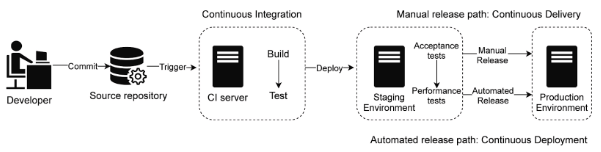
\includegraphics[width=0.9\textwidth]{fig/pipeline1.png}
    \caption{Relaciones entre las prácticas continuas CI, CDE y CD.}
    \label{fig:pipeline1}
\end{figure}
\textbf{DevOps}, una combinación de los términos desarrollo (development) y operaciones (operations), es un enfoque de trabajo que tiene como finalidad  minimizar la desconexión entre los equipos de desarrollo y operaciones mediante la promoción de la colaboración, comunicación y la integración entre ellos \cite{BassDevOpsA2015}. A pesar de ser una tendencia en la industria, DevOps carece de una definición ampliamente aceptada \cite{10.1145/3359981}. Definir DevOps es difícil debido a la considerable superposición con las prácticas continuas \cite{Sthl2017ContinuousPA}. Por esta razón, Stahl et al. \cite{Sthl2017ContinuousPA} presentan definiciones para diferenciar DevOps y prácticas continuas entre sí. En el presente trabajo se considera DevOps compuesto por las prácticas continuas antes mencionadas.

\textbf{DevOps} permite eliminar la barrera que había en una empresa u organización entre los desarrolladores  y  los encargados de las operaciones, permitiendo que se coordinen y colaboren para obtener productos mejores y más confiables. Al adoptar una cultura de DevOps junto a prácticas y herramientas, los equipos adquieren por un lado la  capacidad de responder mejor a las necesidades de los clientes y aumentar la confianza en las aplicaciones que crean y por otro lado alcanzar los objetivos empresariales en menos tiempo. Se emplea el término \textbf{Pipeline} para referirnos al flujo de trabajo y a las tareas a realizar en todas las etapas del desarrollo de software. En la Figura \ref{fig:pipeline2} se ilustran las etapas que componen al pipeline de DevOps.

\begin{figure}[H]
    \centering
    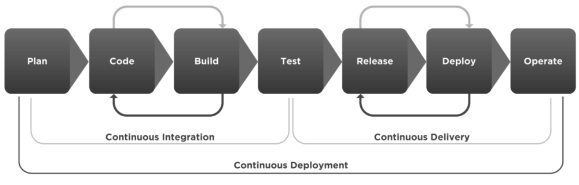
\includegraphics[width=0.9\textwidth]{fig/pipeline2.png}
    \caption{Etapas del Pipeline DevOps.}
    \label{fig:pipeline2}
\end{figure}

Esta nueva forma de trabajar se puede aplicar a los sistemas ciber físicos \textbf{(Cyber Physical Systems, CPS)}, en los cuales se integra la computación, almacenamiento y comunicación junto con capacidades de seguimiento y/o control de objetos en el mundo físico.
Dentro de estos sistemas, se tiene al \textbf{Internet of Things (IoT)}, el cual es un paradigma emergente que permite la comunicación entre dispositivos electrónicos y sensores a través de Internet para facilitar la vida cotidiana. Como ejemplo de IoT se pueden mencionar el \textbf{Smart Home Systems (SHS),} sistemas de automatización para hogares, de administración de energía, etc.


    \chapter{Actividades Desarrolladas}\label{cap:actividades}
En esta sección se incluye una descripción pormenorizada de las actividades desarrolladas durante la Práctica Supervisada.

\section{Objetivos}
\subsection{Objetivo General}
Implementar un Pipeline de DevOps para aplicaciones Internet of Things (IoT) con el dispositivo ESP32.
\subsection{Objetivos Específicos}
\begin{enumerate}
\item Revisión de documentación de DevOps aplicada a IoT.
\item Elegir las herramientas para la construcción del pipeline.
\item Implementar cada etapa que compone el pipeline.
\item Desarrollar una aplicación IoT sencilla utilizando el pipeline implementado.
\item Documentar de forma incremental el trabajo realizado.
\end{enumerate}

\newpage
\section{Metodología}
\subsection{Investigación}
En primer lugar se comenzó investigando sobre la cultura DevOps, las prácticas continuas que se mencionan en el \nameref{cap:marco_teorico}, obteniendo la información a partir de documentación, artículos científicos a los cuales se hace referencia, y la lectura del libro \textit{The DevOps Handbook} \cite{DevOpsHandbook}, que menciona aspectos acerca de cómo surgió esta cultura y cuáles son las problemáticas que viene a solucionar. 

Se siguió además un curso libre y gratuito de prácticas DevOps en YouTube \href{https://www.youtube.com/watch?v=wdFwjWyF47g&list=PLnf4-vBnJ1n1Es3RyaqeIzprp4xUivflP}{(enlace al curso)}, de índole teórico-práctico, que resultó útil para conocer conceptos y herramientas como la \textbf{contenerización con Docker}, la creación de \textbf{Pipelines con GitHub Actions}, entre otras actividades que se detallan en el presente informe. 

\subsection{Dispositivo ESP32}
El dispositivo IoT elegido para trabajar es el \textbf{microcontrolador ESP32}. Se trata de un dispositivo pequeño, de bajo costo y de bajo consumo, cuyas principales prestaciones son la \textbf{conectividad WiFi} y \textbf{Bluetooth}. Su procesador posee 2 núcleos que trabajan a una frecuencia de hasta 240 MHz, entre otras características que se detallan en la siguiente tabla.

\begin{table}[h]
\begin{center}
\begin{tabular}{ll}
\hline
\multicolumn{1}{|l|}{\textbf{Fabricante}} & \multicolumn{1}{l|}{Espressif} \\ \hline
\multicolumn{1}{|l|}{\textbf{Fecha de Lanzamiento}} & \multicolumn{1}{l|}{05/09/2016} \\ \hline
\multicolumn{1}{|l|}{\textbf{Procesador}} & \multicolumn{1}{l|}{Tensilica Xtensa LX6} \\ \hline
\multicolumn{1}{|l|}{\textbf{Frecuencia}} & \multicolumn{1}{l|}{160 MHz (240MHz overclock)} \\ \hline
\multicolumn{1}{|l|}{\textbf{Alimentación}} & \multicolumn{1}{l|}{3.3 VDC} \\ \hline           
\end{tabular}
\caption{Características de ESP32}
\label{tab:car-esp32}
\end{center}
\end{table}

En concreto, este microcontrolador se vende en diferentes placas de desarrollo, con diferencias en los pines de \textbf{General Purpose Input Output (GPIO)}, y diferencias de tamaño. Es decir, se venden diferentes placas que incorporan el mismo microcontrolador ESP32, con diferencias en los pines que disponen.

La placa que se adquirió es la \textbf{“NodeMCU32S”}, que se consigue fácilmente para comprar online y dispone de 35 pines, ideal para trabajar en una protoboard y hacer pruebas. Además, dispone un conector microUSB, para poder conectarse a la PC e implementar el programa.

\begin{figure}[H]
    \centering
    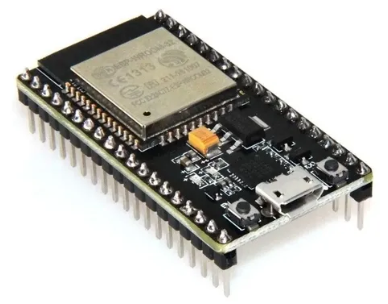
\includegraphics[width=0.6\textwidth]{fig/esp32_1.png}
    \caption{Placa ESP32 tipo NodeMCU32S.}
    \label{fig:esp32_1}
\end{figure}

Para más información sobre este dispositivo se puede consultar su datasheet en el siguiente enlace: \href{https://docs.ai-thinker.com/_media/esp32/docs/nodemcu-32s_product_specification.pdf}{Datasheet NodeMCU32s}

\subsection{Aplicación}
Se construyó una aplicación, lo más sencilla posible, para familiarizarse con la placa, con qué herramientas se puede trabajar, y qué lenguaje de programación resulta la mejor opción para este trabajo.

Se optó por crear el clásico \textbf{LED intermitente}, codificado en \textbf{lenguaje C}, que parpadea a una determinada frecuencia, observable empíricamente en el LED que trae integrado el microcontrolador. 

Cuando se desee hacer un cambio en la aplicación, lo más sencillo será modificar la frecuencia de intermitencia del LED, volver a cargar el código en la placa, y observar el cambio de frecuencia efectuado. A continuación se presenta el código \ref{cod:blinkled} de ejemplo para esta aplicación simple.

\newpage
\begin{lstlisting}[language=C, caption={BlinkLED}, label={cod:blinkled}, captionpos=b]
#include <driver/gpio.h>
// Include FreeRTOS for delay
#include <freertos/FreeRTOS.h>
#include <freertos/task.h>
#define LED 2 // LED connected to GPIO2
#define DELAY 500 // delay in ms to toggle LED state
int app_main() {
    // Configure pin
    gpio_config_t io_conf;
    io_conf.intr_type = GPIO_PIN_INTR_DISABLE;
    io_conf.mode = GPIO_MODE_OUTPUT;
    io_conf.pin_bit_mask = (1ULL << LED);
    io_conf.pull_down_en = 0;
    io_conf.pull_up_en = 0;
    gpio_config(&io_conf);
    // Main loop
    while(true) {
        gpio_set_level(LED, 0);
        vTaskDelay(pdMS_TO_TICKS(DELAY));
        gpio_set_level(LED, 1);
        vTaskDelay(pdMS_TO_TICKS(DELAY));
    }
}
\end{lstlisting}
(Código basado en el ejemplo: \href{https://techoverflow.net/2020/04/09/platformio-esp-idf-esp32-blink-example/}{PlatformIO ESP-IDF ESP32 Blink})

En el código, se observa que las primeras líneas incluyen dependencias importantes de mencionar:
\begin{itemize}
\item \textbf{gpio.h}: Permite acceder a los pines GPIO, y leer o escribir en ellos, entre otras funcionalidades.
\item \textbf{FreeRTOS.h}: Módulo principal del Sistema Operativo de tiempo real \href{https://www.freertos.org/}{FreeRTOS}, que permite gestionar los recursos del microcontrolador y crear tareas con tiempos límites.
\item \textbf{task.h}: Módulo de tareas de FreeRTOS.
\end{itemize}

A partir de la línea 8 del código, se configuran los pines GPIO para poder escribir en el LED integrado de la ESP32, y a partir de la línea 16 se tiene el bucle principal, que se repite indefinidamente, alternando el estado del LED cada \textbf{DELAY [ms]}, en este caso cada 500 [ms] pero puede modificarse fácilmente en la linea 6, es decir en su definición. La función \textbf{pdMS\_TO\_TICKS()}, convierte su parámetro de milisegundos a ticks, que es la manera de contabilizar el tiempo que utiliza \href{https://www.freertos.org/}{FreeRTOS}.

\subsection{PlatformIO}
La primera dificultad encontrada fue al cargar el programa a la placa. Para esta tarea, el fabricante brinda el software, llamado \textbf{Espressif IDF (IoT Development Framework)}, el cual usa scripts de Python para crear y gestionar proyectos. Luego de algunos intentos fallidos, se investigó una herramienta que facilita el proceso de subir el código a la placa, llamada \textbf{PlatformIO}.

\textbf{\href{https://platformio.org/}{PlatformIO}} es un framework destinado al trabajo con dispositivos IoT, soporta aproximadamente 1400 placas de desarrollo, incluyendo la \textbf{ESP32 tipo NodeMCU32S}, que se usa en este proyecto. Se puede instalar como una extensión de \textbf{Visual Studo Code}, uno de los entornos de desarrollo más populares en la actualidad, lo que resulta muy cómodo para trabajar.

Cabe destacar que PlatformIO hace uso del framework Espressif IDF, por lo tanto ayuda a crear una capa de abstracción y facilitar la creación de un proyecto, el acceso a las dependencias, la compilación y la subida del programa al dispositivo con un simple click en el botón \textbf{Build and Upload}.

Gracias a estas facilidades, se logró subir el código del ejemplo \ref{cod:blinkled} con facilidad a la placa. La figura \ref{fig:esp32_2} es una fotografía de la placa haciendo parpadear el LED integrado con éxito.

\begin{figure}[H]
    \centering
    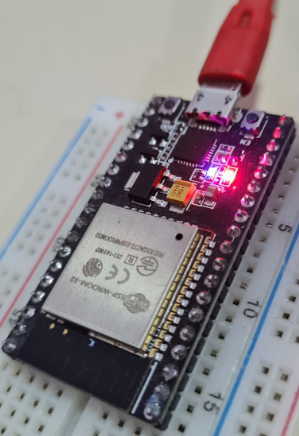
\includegraphics[width=0.5\textwidth]{fig/esp32_2.png}
    \caption{LED intermitente.}
    \label{fig:esp32_2}
\end{figure}

\subsection{Control de Versiones}
Llegado a este punto, es vital contar con una herramienta de control de versiones, para facilitar el trabajo colaborativo y poder volver atrás en caso de introducir errores importantes. Para lograr este objetivo se creó un \textbf{repositorio de Git}, que se aloja en la nube gracias a \textbf{GitHub} o \textbf{GitLab}, las dos plataformas más populares para alojar repositorios de la actualidad.

Con motivos de aprendizaje, se crearon repositorios en ambas plataformas, GitHub y GitLab, ambas son alternativas y el único propósito de subir el mismo contenido a ambas es poder diferenciar las herramientas que ofrece cada una para determinar cuál es mejor para este proyecto.

Luego de investigar y experimentar, \textbf{se decidió continuar con GitHub}, porque resulta más sencillo para aprender e incluye todas las características que necesitamos, siendo la más importante \textbf{GitHub Actions}, que permite crear workflows con secuencias de acciones a ejecutar ante determinados eventos, lo cual se detalla en secciones subsiguientes. 

El repositorio de GitHub se puede encontrar en \url{https://github.com/FeedehC/pipeline-esp32}. Al ingresar al enlace del repositorio se puede ver un README con una guía paso a paso para implementar el pipeline, permitiendo a otros desarrolladores tomar este código y usarlo en sus proyectos IoT. 

Este proyecto es considerado \textbf{Open Source}. Se incentiva la participación haciendo pruebas y realizando aportes, como así también la detección y corrección de errores mediante \textbf{GitHub issues}. 

\subsection{Continuous Integration (CI)}
El próximo paso es añadir CI al proyecto, para esto se usan \textbf{GitHub Actions}, una característica de GitHub que permite crear \textbf{Workflows}.

El término \textbf{Workflow} consiste en un flujo de trabajo, declarado en código YAML, que define distintas tareas (o \textbf{``Jobs"}), ante qué eventos se disparan los Jobs, y qué acciones se llevan a cabo en cada job. Opcionalmente los jobs pueden incluir pasos (o \textbf{``Steps"}) que indican el orden de las instrucciones dentro del job. A su vez, los jobs pueden ejecutarse en paralelo o indicar que para que inicie un job debe terminar otro, y de esta manera ordenar las tareas que se pueden paralelizar y aquellas que deben realizarse en forma secuencial.

En cambio, el término \textbf{Pipeline}, hace alusión a un conjunto de etapas más lineal y más rápido que un Workflow. Sin embargo, en la práctica, es habitual usar estos términos de forma intercambiable. En los párrafos que siguen se usa el término Workflow ya que así se llaman en GitHub Actions.

Una vez creado el Workflow, se indica el evento que lo desencadena. En este caso, el evento es \textbf{cuando se añaden cambios en el código del programa y se pushean a la rama principal} (rama main), a partir del cual se inician una serie de acciones para \textbf{compilar, testear y cargar} automáticamente este código en la placa. De esta misma manera se realiza para entornos de desarrollo Web, con la diferencia de que para proyectos IoT se debe incluir herramientas específicas para cargar el programa en la placa, tal como se detalló anteriormente, con PlatformIO.

\subsection{Descripción del Workflow}
A continuación se presenta una descripción pormenorizada del workflow de GitHub Actions. El mismo se ejecuta cuando se pushean cambios en el contenido de los directorios \textbf{/src} - \textbf{/include} y \textbf{/test}. \textbf{Cualquier cambio que se aplique sobre otra rama o en otras carpetas además de las 3 mencionadas, no ejecutan el pipeline}. Por ejemplo, iniciar el pipeline ante un cambio en la documentación del README, sería innecesario y hasta un desperdicio de recursos. 

\subsubsection{Jobs}
Se optó por crear 3 jobs:
\begin{enumerate}
\item \textbf{Build}: Se encarga de compilar el código con los últimos cambios que se pushearon.
\item \textbf{Test}: Se aplican un conjunto de pruebas al programa antes de cargarlos a la placa.
\item \textbf{Upload}: Se carga el código a la placa.
\end{enumerate}

Cada job precede al anterior, lo que significa que no puede iniciarse hasta que el anterior haya finalizado exitosamente. A continuación se muestra la figura \ref{fig:pipeline3}, un esquema de los jobs y su precedencia.

\begin{figure}[H]
    \centering
    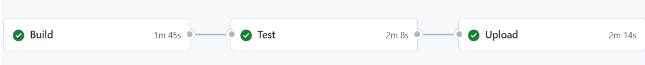
\includegraphics[width=1\textwidth]{fig/pipeline_log.png}
    \caption{Etapas del pipeline}
    \label{fig:pipeline3}
\end{figure}
\subsection{Tests}
Para implementar los tests se hace uso de \href{http://www.throwtheswitch.org/unity}{Unity Tests}, la cual es una herramienta que provee aserciones (o ``\textbf{Asserts}''), que son sentencias que verifican que se cumplan ciertas condiciones en el código. Las pruebas están escritas en lenguaje C y está pensado especialmente para microcontroladores y sistemas embebidos, ya que permite usar macros y otras facilidades para probar estos sistemas durante su desarrollo.

Dentro del proyecto, los tests se ubican en la carpeta \textbf{/test/}, en este caso se tiene sólo un archivo de tests, llamado \href{https://github.com/FeedehC/pipeline-esp32/blob/main/test/test_main.c}{\textbf{test\_main.c}}.

Se crearon 2 tests:
\begin{enumerate}
\item Chequear que $$DELAY >= 50 [ms] $$
Para esta prueba se usa la función \textbf{TEST\_ASSERT\_GREATER\_OR\_EQUAL()}
\item Chequear que $$ DELAY <= 5000 [ms] $$
Para esta prueba se usa la función \textbf{TEST\_ASSERT\_LESS\_OR\_EQUAL()}
\end{enumerate}


A continuación se presenta el código de los tests:

\begin{lstlisting}[language=C, caption={UnityTests}, label={cod:unity-tests}, captionpos=b]
#include <unity.h>
#include "blink.h"
void test_blink_led(void)
{
  //Test if DELAY value is between 50 and 5000 ms
  TEST_ASSERT_GREATER_OR_EQUAL(50, DELAY);
  TEST_ASSERT_LESS_OR_EQUAL(5000, DELAY);
}
int runUnityTests(void)
{
  UNITY_BEGIN();
  RUN_TEST(test_blink_led);
  return UNITY_END();
}
void app_main()
{
  runUnityTests();
}
\end{lstlisting}

Estos tests crean un \textbf{rango válido de valores} para la constante de tiempo DELAY. Recordemos que \textbf{DELAY es el tiempo que tiene que transcurrir para que el LED cambie de estado}, es decir, se encienda si está apagado o viceversa. La idea es que si no se cumple alguna de estas pruebas, el pipeline no continúe su ejecución normal y se evite cargar el código en la placa, simulando una prevención de posibles daños. Además se notifica con un email automático, avisando que falló la ejecución del pipeline cuál de los jobs produjo el fallo, en este caso el job tests.

\textbf{Rango Válido de valores de DELAY:}
 $$50[ms] <= DELAY <= 5000[ms]$$



\newpage
\subsection{Runners}

Cuando se trabaja con pipelines, por defecto las acciones se ejecutan en un servidor en la nube, llamado \textbf{Runner}. Si bien GitHub provee un runner de forma gratuita, está limitado a una cantidad de minutos de ejecución por mes, excedidos estos minutos se solicita facturación. A continuación se presenta la tabla \ref{tab:minutos-gratuitos} con la información de facturación de los runners de GitHub, a modo informativo.

\begin{table}[H]
\begin{center}
\begin{tabular}{lll}
\hline
\multicolumn{1}{|l|}{\textbf{Producto}} & \multicolumn{1}{l|}{\textbf{Almacenamiento}} & \multicolumn{1}{l|}{\textbf{Minutos por mes}} \\ \hline
\multicolumn{1}{|l|}{GitHub Free} & \multicolumn{1}{l|}{500MB} & \multicolumn{1}{l|}{2000} \\ \hline
\multicolumn{1}{|l|}{GitHub Pro} & \multicolumn{1}{l|}{1GB} & \multicolumn{1}{l|}{3000} \\ \hline
\end{tabular}
\caption{Minutos Gratuitos de los GitHub Runners}
\label{tab:minutos-gratuitos}
\end{center}
\end{table}

A su vez, dependiendo del sistema operativo deseado para el runner, se tiene un multiplicador de minutos, que básicamente indica que un minuto de reloj se contabiliza como varios minutos de ejecución del runner, consumiendo más rápidamente la tasa de minutos gratuitos. La tabla \ref{tab:multiplicadores-minutos} detalla los multiplicadores mencionados.

\begin{table}[H]
\begin{center}
\begin{tabular}{lll}
\hline
\multicolumn{1}{|l|}{\textbf{Sistema Operativo}} & \multicolumn{1}{l|}{\textbf{Multiplicador de Minutos}} \\ \hline
\multicolumn{1}{|l|}{Linux} & \multicolumn{1}{l|}{1} \\ \hline
\multicolumn{1}{|l|}{Windows} & \multicolumn{1}{l|}{2} \\ \hline
\multicolumn{1}{|l|}{macOS} & \multicolumn{1}{l|}{10} \\ \hline
\end{tabular}
\caption{Multiplicadores de Minutos de los GitHub Runners}
\label{tab:multiplicadores-minutos}
\end{center}
\end{table}

La facturación del runner se hace en función de cuantos minutos se sobrepasen del límite de minutos gratuitos por mes, lo que se puede ver en la siguiente tabla \ref{tab:costos-minutos} .

\begin{table}[H]
\begin{center}
\begin{tabular}{lll}
\hline
\multicolumn{1}{|l|}{\textbf{Sistema Operativo}} & \multicolumn{1}{l|}{\textbf{Tasa por minuto (USD)}} \\ \hline
\multicolumn{1}{|l|}{Linux} & \multicolumn{1}{l|}{\$0.008} \\ \hline
\multicolumn{1}{|l|}{Windows} & \multicolumn{1}{l|}{\$0.016} \\ \hline
\multicolumn{1}{|l|}{macOS} & \multicolumn{1}{l|}{\$0.08} \\ \hline
\end{tabular}
\caption{Costos de Minutos de los GitHub Runners}
\label{tab:costos-minutos}
\end{center}
\end{table}

(La información acerca de la facturación de GitHub Runners se encuentra en: \href{https://docs.github.com/es/billing/managing-billing-for-github-actions/about-billing-for-github-actions}{Billing for GitHub Actions})

Por este motivo se decidió crear un Runner local, también conocido como \textbf{self-hosted runner}, es decir, brindar la capacidad de cómputo de una computadora propia para permitirle al runner correr las tareas o jobs, evitando usar los recursos de la nube y \textbf{tener un runner disponible de manera gratuita}.

La contraparte de crear un runner local, es que hace falta mantener el servidor que lo ejecuta, instalar actualizaciones y asegurarse que siempre está disponible.

Luego de seguir las instrucciones para levantar el runner local, se tuvo el inconveniente de que no funciona en algunas distribuciones de Linux, debido a un error de dependencias de módulos de Python. Para solucionar este problema, \textbf{se corre el self-hosted runner dentro de un contenedor de Docker}, que se detalla en la siguiente sección.

\subsection{Docker}

\href{https://www.docker.com/}{Docker} es una herramienta popular en la cultura DevOps, que permite crear contenedores que encapsulan las dependencias que requiere una aplicación para correr.

Los \textbf{contenedores} son piezas de software livianas, independientes, empaquetables y ejecutables que incluyen todo lo que necesita para correr las aplicaciones: código, herramientas de sistema, librerías y configuraciones. Cabe aclarar que un contenedor se ejecuta como un proceso independiente dentro de un sistema operativo por consiguiente puede ser afectado por el controlador de procesos del sistema operativo.

Por otro lado, una \textbf{imagen} de Docker, es una receta para poder instanciar contenedores, tantos como sean necesarios de la misma aplicación. La imagen está descrita en un archivo llamado \textbf{Dockerfile}, dentro de este archivo se encuentran todas las capas necesarias para construir la imagen. A su vez las imágenes tienen un tag o etiqueta que permite versionarlas.

Hasta este punto se tiene una imagen construida y un contenedor creado a partir de la imagen, ejecutándose en la máquina local. Sin embargo, la potencia de los contenedores se presenta a la hora de realizar despliegues (o ``\textbf{Deployments}'') de las aplicaciones en diferentes entornos. Para esto se tiene un nuevo concepto llamado \textbf{registro}. \textbf{Docker registry} es un repositorio donde se almacenan imágenes de Docker. La versión comercial se encuentra en \href{https://hub.docker.com}{Dockerhub}.

La figura \ref{fig:docker} muestra un esquema en el que se ilustran los conceptos mencionados anteriormente, además de los comandos de Docker, y también aparece el \textbf{Docker daemon}, que es el proceso encargado de gestionar las imágenes y contenedores. Por otro lado, el registry representa un repositorio en la nube, al que se pueden subir o bajar imágenes.

\begin{figure}[H]
    \centering
    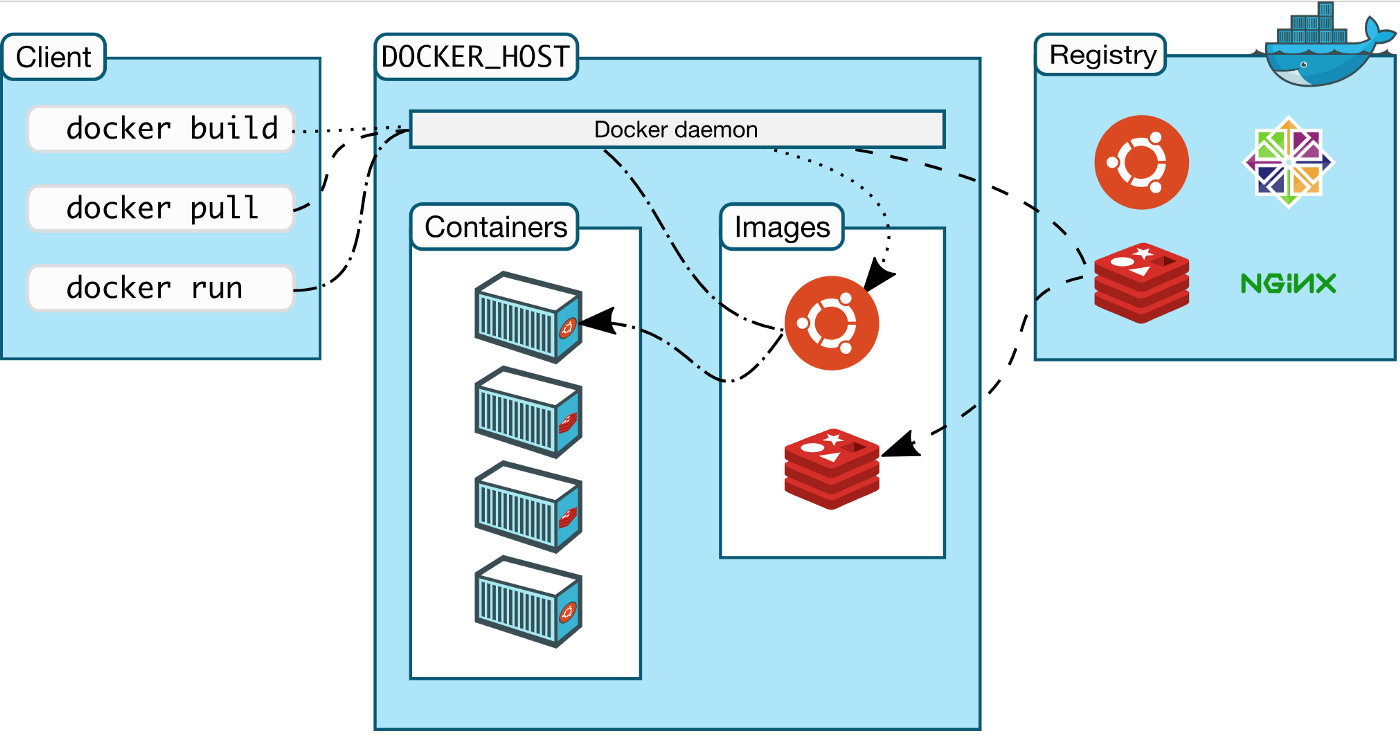
\includegraphics[width=1\textwidth]{fig/docker.png}
    \caption{Docker: Esquema de los conceptos}
    \label{fig:docker}
\end{figure}

(La figura \ref{fig:docker} es propiedad intelectual de Mauricio Collazos, y su post se encuentra en este \href{https://medium.com/ingenier%C3%ADa-en-tranqui-finanzas/una-gu%C3%ADa-no-tan-r%C3%A1pida-de-docker-y-kubernetes-933f5b6709df } {enlace} )

Gracias a la tecnología de los contenedores, podemos abstraernos del sistema en el  que se corre la aplicación, y dar solución al problema de que la aplicación funciona en algunos sistemas y no en otros, típicamente por problemas en sus dependencias.

En concreto, se partió de la imagen \href{https://registry.hub.docker.com/r/tcardonne/github-runner}{GitHub Runner de TCardonne} para crear un \textbf{self-hosted runner pero esta vez encapsulado en un contenedor}.

\subsubsection{Docker Compose}

Para facilitar la inicialización del contenedor se usa \href{https://docs.docker.com/compose/}{Docker Compose}, que es una herramienta para declarar como código YAML uno o más contenedores para instanciarse, desde qué imagen se parte, y su configuracion específica, como el mapeo de puertos con el sistema host, si posee o no un volumen asociado, redes, entre otras. 

Gracias a esta herramienta, basta con ejecutar el comando \textbf{sudo docker-compose up} para iniciar el contenedor correspondiente al self-hosted runner. Cabe aclarar que Docker Compose no agrega funcionalidad más allá de Docker, sino que permite declarar como código las configuraciones que de otra forma tendrían que hacerse con los comandos de docker: \textbf{docker pull, docker build, docker run} como se muestran en la figura \ref{fig:docker}. Este código se encuentra en el archivo \href{https://github.com/FeedehC/pipeline-esp32/blob/main/docker-compose.yml}{docker-compose.yml} ubicado en el directorio raíz del proyecto.

Una vez que está corriendo el contenedor de Docker con el self-hosted runner, el mismo está ``escuchando jobs", lo que significa que está a la espera de que un evento dispare la ejecución del pipeline, es decir, que un desarrollador haga un push que involucre cambios en el código, en este caso un cambio en la frecuencia de intermitencia del LED.

A continuación se presenta una captura de pantalla de la terminal que corre el contenedor con el runner, en la figura \ref{fig:runner}.

\begin{figure}[H]
    \centering
    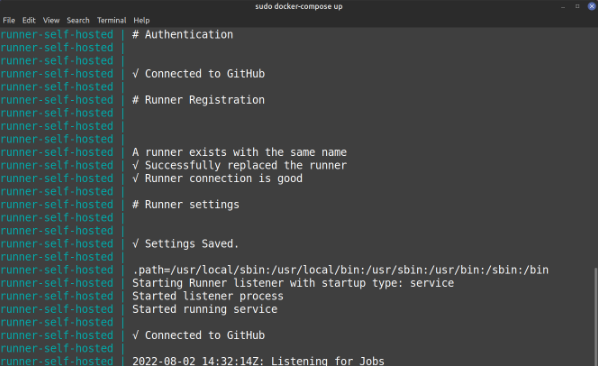
\includegraphics[width=1\textwidth]{fig/runner_log.png}
    \caption{GitHub Self-Hosted Runner}
    \label{fig:runner}
\end{figure}


\subsection{Documentación}
Una vez logrado el pipeline y su ejecución exitosa, se documentó el trabajo, confeccionando el presente informe de las actividades llevadas a cabo, y además el README del \href{https://github.com/FeedehC/pipeline-esp32}{repositorio de GitHub} que indica paso a paso como crear una copia personal con el repositorio proyecto, es decir, un \textbf{``fork''}, y como implementar el pipeline para un proyecto personal. 

Si bien el proyecto está configurado para trabajar con una placa \textbf{ESP32 tipo NodeMCU32s}, en caso que otros desarrolladores necesiten implementar el pipeline para un proyecto que usa otro dispositivo, y considerando que el dispositivo es soportado por PlatformIO (lo que se puede verificar en el siguiente \href{https://registry.platformio.org/search?t=platform}{enlace}), bastará con ajustar las configuraciones en el archivo \href{https://github.com/FeedehC/pipeline-esp32/blob/main/platformio.ini}{\textbf{platformio.ini}} ubicado en la carpeta raíz del repositorio. Es en este archivo donde se detallan los ajustes de PlatformIO y es posible incluso declarar más de un entorno de trabajo, es decir, trabajar con distintos dispositivos e indicar qué dependencias corresponden a cada uno. 

Para subir el código a un dispositivo u otro, se debe aclarar el \textbf{environment} al momento de ejecutar el comando \textbf{pio run}, típicamente en el archivo \href{https://github.com/FeedehC/pipeline-esp32/blob/main/.github/workflows/main.yml}{\textbf{.github/workflows/main.yml}}, es decir, en el código YAML del pipeline.

Como extra \textbf{se añadió una versión en inglés de la documentación} del repositorio, que se puede encontrar en el archivo \href{https://github.com/FeedehC/pipeline-esp32/blob/main/README-english.md}{\textbf{README-english.md}} en la raíz del repositorio, con el propósito de poder compartirlo con desarrolladores que prefieran esta lengua para trabajar.


    \chapter{Conclusiones}\label{cap:conclusiones}
Una vez finalizado el trabajo, con el self-hosted runner contenerizado con Docker, y teniendo el microcontrolador conectado por cable microUSB a la computadora que actúa como servidor para correr el runner, se está en condiciones de modificar el código del programa desde cualquier lugar con acceso a internet. En esta aplicación sencilla se espera únicamente un cambio en la frecuencia de parpadeo del LED.

Una vez que se pushean al repositorio cambios en las carpetas /src, /include y /tests de la rama principal, se desencadenan las tareas del Workflow para compilar, testear y cargar el nuevo programa en la placa.

\textbf{Consumo de Recursos}

Se midió el consumo de recursos de esta aplicación sencilla para la placa, gracias a la funcionalidad de PlatformIO Statistics, obteniendo las métricas de uso de memoria RAM, uso de almacenamiento Flash, y defectos encontrados, las cuales se muestran en la figura \ref{fig:metrics}.

\begin{figure}[H]
    \centering
    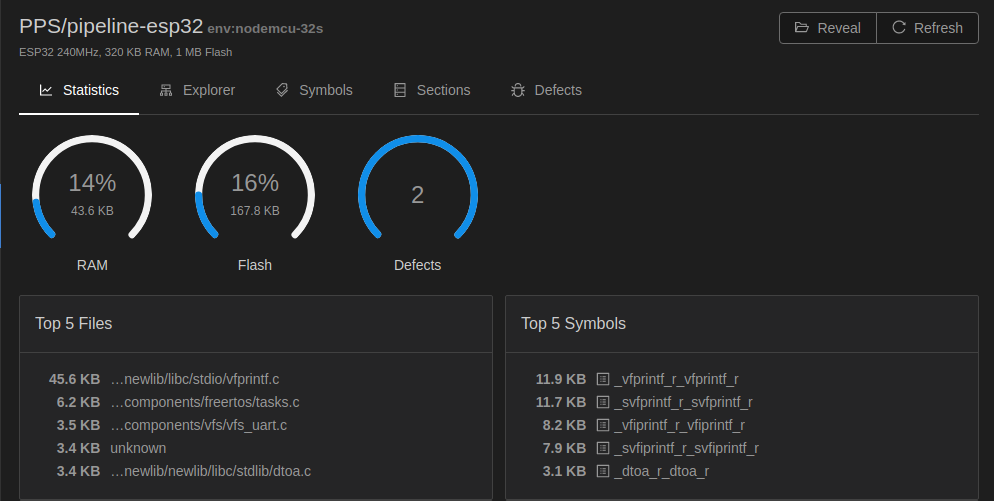
\includegraphics[width=1\textwidth]{fig/platformio-esp32-metrics.png}
    \caption{Métricas del ESP32 corriendo la aplicación}
    \label{fig:metrics}
\end{figure}

\textbf{Tiempos}

La ejecución inicial del runner demora aproximadamente 2 minutos hasta que está listo para ejecutar jobs.
Cuando se pushea un cambio por primera vez, se demora bastante para instalar las dependencias en el contenedor, aproximadamente unos 8 minutos. Para posteriores pusheos de cambios, se corren los jobs más rápidamente porque el contenedor ya tiene sus dependencias instaladas, en este caso demora aproximadamente 2 minutos en cargar el nuevo código en la placa, considerando que pasaron exitosamente los tests. Se resume esta información en la tabla

\begin{table}[H]
\begin{center}
\begin{tabular}{lll}
\hline
\multicolumn{1}{|l|}{\textbf{Caso}} & \multicolumn{1}{l|}{\textbf{Tiempo aproximado}} \\ \hline
\multicolumn{1}{|l|}{Ejecución Inicial del Runner con Docker} & \multicolumn{1}{l|}{2 minutos} \\ \hline
\multicolumn{1}{|l|}{Workflow Jobs al recibir el primer push} & \multicolumn{1}{l|}{8 Minutos} \\ \hline
\multicolumn{1}{|l|}{Workflow Jobs al recibir los siguientes pushes} & \multicolumn{1}{l|}{2 Minutos} \\ \hline
\end{tabular}
\caption{Tiempos del GitHub Runner en ejecutar las tareas del Workflow}
\label{tab:multiplicadores-minutos}
\end{center}
\end{table}

Los tiempos dependen de la computadora con la que se corre el self-hosted runner, en este caso se trata de una notebook de gama media del año 2020, modelo Lenovo Legión 5i, cuya ficha técnica se puede encontrar en el siguiente \href{https://www.lenovo.com/ar/es/laptops/laptops-legion/legion-5-series/Legion-5i-15/p/88GMY501434}{enlace}.



    %\chapter{Ejemplos de uso LaTeX}\label{cap:ejemplos}

\todo[inline]{Este capítulo se incluye únicamente como ayuda y referencia de uso de \LaTeX. No debe aparecer en el documento final.}

\section{Introducción}
En este capítulo se muestran ejemplos de uso de \LaTeX para operaciones comunes. 

\section{Estilos}\label{sec:estilos}
Se pueden aplicar estilos al texto como \textbf{negritas}, \textit{cursiva} y \underline{subrayado}. También se \textcolor{red}{pueden} \textcolor{blue}{aplicar} \textcolor{green}{colores}, y \underline{\textit{combinar}} \textbf{\textcolor{red}{estilos}}. Se recomienda usar sólo negritas para hacer énfasis, y no abusar de este recurso.

\section{Listados}
Con itemize se pueden crear listas no numeradas:

\begin{itemize}
    \item Fresas
    \item Melocotones
    \item Piñas
    \item Nectarinas
\end{itemize}

De manera similar, enumerate permite crear listas numeradas:

\begin{enumerate}
    \item Elaborar la memoria del TFG
    \item Elaborar la presentación
    \item Presentar el TFG
    \item Solicitar el título de Grado
\end{enumerate}

\section{Subsecciones}
Se pueden definir subsecciones con el comando subsection:

\subsection{Primera subsección}\label{sec:subseccion}
Esto es una subsección

\subsection{Segunda subsección}
Esto es otra subsección.

\section{Imágenes y figuras}
Todas las imágenes y figuras del documento se incluirán en la carpeta ``fig''. Se pueden incluir de la siguiente manera:

\begin{figure}[htp]
    \centering
    
\includegraphics[width=0.7\textwidth]{fig/ejemplo.png}
    \caption{Un feroz depredador}
    \label{fig:ejemplo}
\end{figure}

Observe que las figuras se numeran automáticamente según el capítulo y el número de figuras que hayan aparecido anteriormente en dicho capítulo. Existen muchas maneras de definir el tamaño de una figura, pero se aconseja utilizar la mostrada en este ejemplo: se define el ancho de la figura como un porcentaje del ancho total de la página, y la altura se escala automáticamente. De esta manera, el ancho máximo de una figura sería 1.0 * textwidth, lo que aseguraría que se muestra al máximo tamaño posible sin sobrepasar los márgenes del documento.

Tenga en cuenta que LaTeX intenta incluir las figuras en el mismo sitio donde se declaran, pero en ocasiones no es posible por motivos de espacio. En esos casos, LaTeX colocará la figura lo más cerca posible de su declaración, puede que en una página diferente. Esto es un comportamiento normal y no debe ser evitado.

\section{Referencias}
Observe cómo en el código fuente de esta sección se ha usado varias veces el comando ``label''. Este comando permite marcar un elemento, ya sea capítulo, sección, figura, etc. para hacer una referencia numérica al mismo. Para referenciar una ``label'' se usa el comando ``ref'' incluyendo el nombre de la referencia:

Este es el capítulo \ref{cap:ejemplos}.

En la sección \ref{sec:estilos} se muestran ejemplos de estilos.

La subsección \ref{sec:subseccion} explica...

En la Figura \ref{fig:ejemplo} vemos que...

Esto evita que tengamos que escribir directamente los índices de las secciones y figuras que queremos mencionar, ya que LaTeX lo hace por nosotros y además se encarga de mantenerlos actualizados en caso de que cambien (pruebe a mover este capítulo al final del documento y observe cómo se actualizan automáticamente todos los índices referenciados). Además, las referencias mediante ``ref'' actúan como hipervínculos dentro del documento que llevan al elemento referenciado al pulsar en ellas.

Es habitual nombrar las ``label'' con un prefijo que indica el tipo de elemento para encontrarlo luego más fácilmente, pero no es obligatorio.

\section{Extractos de código}

Se pueden incluir extractos de código mediante lstlisting:

\begin{lstlisting}[language=Python, caption={Código Python}, label={cod:python}, captionpos=b]
num = float(input("Enter a number: "))
if num > 0:
   print("Positive number")
elif num == 0:
   print("Zero")
else:
   print("Negative number")
\end{lstlisting}

Se admite gran variedad de lenguajes:

\begin{lstlisting}[language=Java, caption={Código Java}, label={cod:java}, captionpos=b]
public class Test {
    public static void main(String[] args) {
        System.out.println("Hello, world!");
    }
}
\end{lstlisting}

Los extractos de código también se pueden referenciar mediante label/ref: Extractos de código \ref{cod:python} y \ref{cod:java}.

\section{Enlaces}
Puede enlazar una web externa mediante el comando url: \url{https://www.example.com}. También se puede vincular un enlace a un texto mediante el comando href: \href{https://www.example.com}{dominio de ejemplo}.

\section{Citas y bibliografía}
En LaTeX, los elementos de la bibliografía se almacenan en un fichero bibliográfico en un formato llamado BibTeX, en el caso de este proyecto se encuentran en ``bibliografia.bib''. Para citar un elemento se usa el comando ``cite''. Se pueden citar tanto artículos científicos \cite{borrego2019} como enlaces web \cite{webETSII}. 

También se puede usar el comando ``citet'' para incluir una referencia junto con el nombre de su autor o autores: \citet{borrego2021}. Todas las citas se numeran automáticamente y se incluyen en la sección de bibliografía del documento.

Observe cómo los elementos bibliográficos almacenados en ``bibliografia.bib'' tienen una etiqueta asociada, que es la que se incluye al citarlos mediante cite. Añadir una referencia al fichero bibliográfico no hace que ésta aparezca automáticamente en la sección de bibliografía del trabajo, es necesario citarla en algún lugar del mismo.

\section{Ecuaciones}
LaTeX tiene un potente motor para mostrar ecuaciones matemáticas y un amplio catálogo de símbolos matemáticos. El entorno matemático se puede activar de muchas maneras. Para incluir ecuaciones simples en un texto se pueden rodear de símbolos dólar: $1 + 2 = 3$, $\sqrt{81} = 3^2 = 9$, $\forall x \in y~\exists~z : S_z < 4$.

Las ecuaciones más complejas pueden expresarse aparte y son numeradas: ecuación \ref{eq:ecuacion}.

\begin{equation}\label{eq:ecuacion}
\lim_{x\to 0}{\frac{e^x-1}{2x}}
 \overset{\left[\frac{0}{0}\right]}{\underset{\mathrm{H}}{=}}
 \lim_{x\to 0}{\frac{e^x}{2}}={\frac{1}{2}}
 +7 \int_0^2
  \left(
    -\frac{1}{4}\left(e^{-4t_1}+e^{4t_1-8}\right)
  \right)\,dt_1
\end{equation}

Dispone \href{http://www.yann-ollivier.org/latex/texsymbols.pdf}{aquí} de un amplio listado de símbolos que pueden usarse en modo matemático.

\section{Caracteres y símbolos especiales}
Algunos caracteres y símbolos deben ser escapados para poder representarse en el documento, ya que tienen un significado especial en LaTeX. Algunos de ellos son:

\begin{itemize}
    \item El símbolo dólar \$ se usa para ecuaciones.
    \item El tanto por ciento \% se usa para comentarios en el código fuente.
    \item El símbolo euro \euro{} suele dar problemas si se escribe directamente.
    \item El guión bajo \_ se usa para subíndices en modo matemático.
    \item Las comillas deben expresarse `así' para comillas simples y ``así'' para comillas dobles. Las comillas españolas pueden expresarse \textquote{así}.
    \item La barra invertida o contrabarra \textbackslash{} se usa para comandos LaTeX.
    \item Otros símbolos que deben escaparse son las llaves \{ \}, el ampersand \&, la almohadilla \# y los símbolos mayor que \textgreater{} y menor que \textless{}.
\end{itemize}
    
    % Bibliografía
    \bibliographystyle{plainnat}
    \bibliography{bibliografia.bib}

% Fin del documento
\end{document}
